% Options for packages loaded elsewhere
\PassOptionsToPackage{unicode}{hyperref}
\PassOptionsToPackage{hyphens}{url}
%
\documentclass[
]{article}
\usepackage{amsmath,amssymb}
\usepackage{iftex}
\ifPDFTeX
  \usepackage[T1]{fontenc}
  \usepackage[utf8]{inputenc}
  \usepackage{textcomp} % provide euro and other symbols
\else % if luatex or xetex
  \usepackage{unicode-math} % this also loads fontspec
  \defaultfontfeatures{Scale=MatchLowercase}
  \defaultfontfeatures[\rmfamily]{Ligatures=TeX,Scale=1}
\fi
\usepackage{lmodern}
\ifPDFTeX\else
  % xetex/luatex font selection
\fi
% Use upquote if available, for straight quotes in verbatim environments
\IfFileExists{upquote.sty}{\usepackage{upquote}}{}
\IfFileExists{microtype.sty}{% use microtype if available
  \usepackage[]{microtype}
  \UseMicrotypeSet[protrusion]{basicmath} % disable protrusion for tt fonts
}{}
\makeatletter
\@ifundefined{KOMAClassName}{% if non-KOMA class
  \IfFileExists{parskip.sty}{%
    \usepackage{parskip}
  }{% else
    \setlength{\parindent}{0pt}
    \setlength{\parskip}{6pt plus 2pt minus 1pt}}
}{% if KOMA class
  \KOMAoptions{parskip=half}}
\makeatother
\usepackage{xcolor}
\usepackage[margin=1in]{geometry}
\usepackage{color}
\usepackage{fancyvrb}
\newcommand{\VerbBar}{|}
\newcommand{\VERB}{\Verb[commandchars=\\\{\}]}
\DefineVerbatimEnvironment{Highlighting}{Verbatim}{commandchars=\\\{\}}
% Add ',fontsize=\small' for more characters per line
\usepackage{framed}
\definecolor{shadecolor}{RGB}{248,248,248}
\newenvironment{Shaded}{\begin{snugshade}}{\end{snugshade}}
\newcommand{\AlertTok}[1]{\textcolor[rgb]{0.94,0.16,0.16}{#1}}
\newcommand{\AnnotationTok}[1]{\textcolor[rgb]{0.56,0.35,0.01}{\textbf{\textit{#1}}}}
\newcommand{\AttributeTok}[1]{\textcolor[rgb]{0.13,0.29,0.53}{#1}}
\newcommand{\BaseNTok}[1]{\textcolor[rgb]{0.00,0.00,0.81}{#1}}
\newcommand{\BuiltInTok}[1]{#1}
\newcommand{\CharTok}[1]{\textcolor[rgb]{0.31,0.60,0.02}{#1}}
\newcommand{\CommentTok}[1]{\textcolor[rgb]{0.56,0.35,0.01}{\textit{#1}}}
\newcommand{\CommentVarTok}[1]{\textcolor[rgb]{0.56,0.35,0.01}{\textbf{\textit{#1}}}}
\newcommand{\ConstantTok}[1]{\textcolor[rgb]{0.56,0.35,0.01}{#1}}
\newcommand{\ControlFlowTok}[1]{\textcolor[rgb]{0.13,0.29,0.53}{\textbf{#1}}}
\newcommand{\DataTypeTok}[1]{\textcolor[rgb]{0.13,0.29,0.53}{#1}}
\newcommand{\DecValTok}[1]{\textcolor[rgb]{0.00,0.00,0.81}{#1}}
\newcommand{\DocumentationTok}[1]{\textcolor[rgb]{0.56,0.35,0.01}{\textbf{\textit{#1}}}}
\newcommand{\ErrorTok}[1]{\textcolor[rgb]{0.64,0.00,0.00}{\textbf{#1}}}
\newcommand{\ExtensionTok}[1]{#1}
\newcommand{\FloatTok}[1]{\textcolor[rgb]{0.00,0.00,0.81}{#1}}
\newcommand{\FunctionTok}[1]{\textcolor[rgb]{0.13,0.29,0.53}{\textbf{#1}}}
\newcommand{\ImportTok}[1]{#1}
\newcommand{\InformationTok}[1]{\textcolor[rgb]{0.56,0.35,0.01}{\textbf{\textit{#1}}}}
\newcommand{\KeywordTok}[1]{\textcolor[rgb]{0.13,0.29,0.53}{\textbf{#1}}}
\newcommand{\NormalTok}[1]{#1}
\newcommand{\OperatorTok}[1]{\textcolor[rgb]{0.81,0.36,0.00}{\textbf{#1}}}
\newcommand{\OtherTok}[1]{\textcolor[rgb]{0.56,0.35,0.01}{#1}}
\newcommand{\PreprocessorTok}[1]{\textcolor[rgb]{0.56,0.35,0.01}{\textit{#1}}}
\newcommand{\RegionMarkerTok}[1]{#1}
\newcommand{\SpecialCharTok}[1]{\textcolor[rgb]{0.81,0.36,0.00}{\textbf{#1}}}
\newcommand{\SpecialStringTok}[1]{\textcolor[rgb]{0.31,0.60,0.02}{#1}}
\newcommand{\StringTok}[1]{\textcolor[rgb]{0.31,0.60,0.02}{#1}}
\newcommand{\VariableTok}[1]{\textcolor[rgb]{0.00,0.00,0.00}{#1}}
\newcommand{\VerbatimStringTok}[1]{\textcolor[rgb]{0.31,0.60,0.02}{#1}}
\newcommand{\WarningTok}[1]{\textcolor[rgb]{0.56,0.35,0.01}{\textbf{\textit{#1}}}}
\usepackage{longtable,booktabs,array}
\usepackage{calc} % for calculating minipage widths
% Correct order of tables after \paragraph or \subparagraph
\usepackage{etoolbox}
\makeatletter
\patchcmd\longtable{\par}{\if@noskipsec\mbox{}\fi\par}{}{}
\makeatother
% Allow footnotes in longtable head/foot
\IfFileExists{footnotehyper.sty}{\usepackage{footnotehyper}}{\usepackage{footnote}}
\makesavenoteenv{longtable}
\usepackage{graphicx}
\makeatletter
\def\maxwidth{\ifdim\Gin@nat@width>\linewidth\linewidth\else\Gin@nat@width\fi}
\def\maxheight{\ifdim\Gin@nat@height>\textheight\textheight\else\Gin@nat@height\fi}
\makeatother
% Scale images if necessary, so that they will not overflow the page
% margins by default, and it is still possible to overwrite the defaults
% using explicit options in \includegraphics[width, height, ...]{}
\setkeys{Gin}{width=\maxwidth,height=\maxheight,keepaspectratio}
% Set default figure placement to htbp
\makeatletter
\def\fps@figure{htbp}
\makeatother
\setlength{\emergencystretch}{3em} % prevent overfull lines
\providecommand{\tightlist}{%
  \setlength{\itemsep}{0pt}\setlength{\parskip}{0pt}}
\setcounter{secnumdepth}{-\maxdimen} % remove section numbering
\ifLuaTeX
  \usepackage{selnolig}  % disable illegal ligatures
\fi
\usepackage{bookmark}
\IfFileExists{xurl.sty}{\usepackage{xurl}}{} % add URL line breaks if available
\urlstyle{same}
\hypersetup{
  pdftitle={OTDM - Constrained Optimization - SVM},
  pdfauthor={Julian Fransen, Danila Kokin},
  hidelinks,
  pdfcreator={LaTeX via pandoc}}

\title{OTDM - Constrained Optimization - SVM}
\author{Julian Fransen, Danila Kokin}
\date{2024-11-24}

\begin{document}
\maketitle

{
\setcounter{tocdepth}{3}
\tableofcontents
}
\begin{Shaded}
\begin{Highlighting}[]
\NormalTok{tinytex}\SpecialCharTok{::}\FunctionTok{tlmgr}\NormalTok{(}\StringTok{"option repository https://mirror.ctan.org/systems/texlive/tlnet"}\NormalTok{)}
\end{Highlighting}
\end{Shaded}

\begin{verbatim}
## tlmgr option repository https://mirror.ctan.org/systems/texlive/tlnet
\end{verbatim}

\begin{enumerate}
\def\labelenumi{\arabic{enumi}.}
\tightlist
\item
  A cover page with the name of the two (and exactly two!) members of
  the group
\end{enumerate}

put a picture of UPC maybe? we have to knit to pdf i think

\begin{titlepage}
    \centering
    \vspace*{4cm} % Adjust vertical spacing
    
\includegraphics[width=\textwidth]{./UPC.jpg}
    \vfill
    {\Huge \textbf{OTDM Lab assignment 3: Cluster median.}} \\[1.5cm]
    {\Large Authors: Julian Fransen, Danila Kokin} \\[0.5cm]
    {\Large Date: \today}
    \vfill
\end{titlepage}

\subsection{2. Description of Data Matrix
A}\label{description-of-data-matrix-a}

\subsubsection{Title: Wine Data (Adapted for Unsupervised
Learning)}\label{title-wine-data-adapted-for-unsupervised-learning}

\subsubsection{Sources:}\label{sources}

\begin{itemize}
\tightlist
\item
  \textbf{Original Source}: UCI Machine Learning Repository
\item
  \textbf{Original Dataset}:
  \href{https://archive.ics.uci.edu/ml/datasets/wine}{Wine Dataset}
\item
  \textbf{Creator}: Forina et al.~(1991), Analytical Chemistry
\end{itemize}

\subsubsection{Relevant Information:}\label{relevant-information}

These data are the results of a chemical analysis of wines grown in the
same region in Italy, derived from three different cultivars. The
analysis determined the quantities of 13 constituents found in each of
the three types of wines. The dataset is adapted for unsupervised
learning by removing the labels that classify the types of wines.

\begin{itemize}
\tightlist
\item
  \textbf{Data Usage}: Frequently used for clustering, PCA, and
  classification studies.
\item
  \textbf{Domain}: Chemistry, wine analysis, and machine learning.
\end{itemize}

\subsubsection{Number of Instances:}\label{number-of-instances}

\begin{itemize}
\tightlist
\item
  178 wine samples.
\end{itemize}

\subsubsection{Number of Attributes:}\label{number-of-attributes}

\begin{itemize}
\tightlist
\item
  13 numeric continuous attributes.
\end{itemize}

\subsubsection{Attribute Information:}\label{attribute-information}

\begin{enumerate}
\def\labelenumi{\arabic{enumi}.}
\tightlist
\item
  Alcohol
\item
  Malic acid
\item
  Ash
\item
  Alcalinity of ash
\item
  Magnesium
\item
  Total phenols
\item
  Flavanoids
\item
  Nonflavanoid phenols
\item
  Proanthocyanins
\item
  Color intensity
\item
  Hue
\item
  OD280/OD315 of diluted wines
\item
  Proline
\end{enumerate}

\subsubsection{Missing Attribute
Values:}\label{missing-attribute-values}

\begin{itemize}
\tightlist
\item
  None.
\end{itemize}

\subsubsection{Preprocessing:}\label{preprocessing}

The dataset was scaled using Z-score normalization to standardize the
features to zero mean and unit variance for better interpretability and
clustering performance. After scaling, the Euclidean distance was
calculated, and this matrix of distances was formatted to AMPL
compatible .dat files.

\subsubsection{Summary Statistics:}\label{summary-statistics}

\begin{longtable}[]{@{}
  >{\raggedright\arraybackslash}p{(\columnwidth - 8\tabcolsep) * \real{0.4143}}
  >{\raggedleft\arraybackslash}p{(\columnwidth - 8\tabcolsep) * \real{0.1000}}
  >{\raggedleft\arraybackslash}p{(\columnwidth - 8\tabcolsep) * \real{0.1143}}
  >{\raggedleft\arraybackslash}p{(\columnwidth - 8\tabcolsep) * \real{0.1000}}
  >{\raggedleft\arraybackslash}p{(\columnwidth - 8\tabcolsep) * \real{0.2714}}@{}}
\toprule\noalign{}
\begin{minipage}[b]{\linewidth}\raggedright
Feature
\end{minipage} & \begin{minipage}[b]{\linewidth}\raggedleft
Min
\end{minipage} & \begin{minipage}[b]{\linewidth}\raggedleft
Max
\end{minipage} & \begin{minipage}[b]{\linewidth}\raggedleft
Mean
\end{minipage} & \begin{minipage}[b]{\linewidth}\raggedleft
Standard Deviation
\end{minipage} \\
\midrule\noalign{}
\endhead
\bottomrule\noalign{}
\endlastfoot
Alcohol & 11.03 & 14.83 & 13.00 & 0.81 \\
Malic acid & 0.74 & 5.80 & 2.34 & 1.12 \\
Ash & 1.36 & 3.23 & 2.36 & 0.27 \\
Alcalinity of ash & 10.60 & 30.00 & 19.49 & 3.34 \\
Magnesium & 70.00 & 162.00 & 99.74 & 14.28 \\
Total phenols & 0.98 & 3.88 & 2.29 & 0.63 \\
Flavanoids & 0.34 & 5.08 & 2.03 & 0.99 \\
Nonflavanoid phenols & 0.13 & 0.66 & 0.36 & 0.12 \\
Proanthocyanins & 0.41 & 3.58 & 1.59 & 0.57 \\
Color intensity & 1.28 & 13.00 & 4.71 & 2.43 \\
Hue & 0.48 & 1.71 & 0.96 & 0.23 \\
OD280/OD315 of diluted wines & 1.27 & 4.00 & 2.61 & 0.71 \\
Proline & 278.00 & 1680.00 & 746.89 & 314.91 \\
\end{longtable}

\subsection{\texorpdfstring{3. The AMPL \texttt{.mod} and \texttt{.dat}
Files}{3. The AMPL .mod and .dat Files}}\label{the-ampl-.mod-and-.dat-files}

\subsubsection{\texorpdfstring{Sample of \texttt{wine.dat}
File:}{Sample of wine.dat File:}}\label{sample-of-wine.dat-file}

\begin{Shaded}
\begin{Highlighting}[]
\NormalTok{param m := 178;}
\NormalTok{param k := 3;}
\NormalTok{param d: 1 2 ... 177 178 :=}
\NormalTok{1   0.000000  3.497535 ...  6.078781  7.184421}
\NormalTok{2   3.497535  0.000000 ...  6.094927  7.367719}
\NormalTok{... }
\NormalTok{178 7.184421  7.367719 ...  3.324276  0.000000;}
\end{Highlighting}
\end{Shaded}

\subsubsection{\texorpdfstring{Contents of \texttt{clustering.mod}
file:}{Contents of clustering.mod file:}}\label{contents-of-clustering.mod-file}

\begin{Shaded}
\begin{Highlighting}[]
\NormalTok{/\#Below we define the AMPL model for clustering}
\NormalTok{param m;}
\NormalTok{param k;}
\NormalTok{param d\{1..m, 1..m\};}
\NormalTok{var x\{1..m, 1..m\} binary;}

\NormalTok{minimize f: sum\{i in 1..m, j in 1..m\} d[i,j]*x[i,j];}
\NormalTok{subject to c1\{i in 1..m\}: sum\{j in 1..m\} x[i,j] = 1;}
\NormalTok{/\# This constraint ensures every point belongs to 1 cluster}
\NormalTok{subject to c2: sum\{j in 1..m\} x[j,j] = k;}
\NormalTok{/\# This constraint ensure that there are exactly k clusters}
\NormalTok{subject to c3\{i in 1..m, j in 1..m\}: x[j,j] \textgreater{}= x[i,j];}
\NormalTok{/\# This constraint ensures that a point can only be part of a cluster that exists}
\end{Highlighting}
\end{Shaded}

\subsection{4. The optimal solution obtained with
AMPL.}\label{the-optimal-solution-obtained-with-ampl.}

\#```\{bash, echo=FALSE\} cd
/home/julian/uni\_folder/OTDM/OTDM\_Project\_2/3/linprog/
/home/julian/uni\_folder/OTDM/OTDM\_p2/OTDM/ampl\_linux-intel64/ampl
\textless\textless{} EOF

reset; reset data;

model clustering.mod; data wine2.dat; option solver cplex; option
cplex\_options `timing 1'; solve;

print '' Matrix x (formulation)``; print''\,``;

print '' Number of points per cluster''; print ``\,``;

var total\{i in 1..m\};

for \{i in 1..m\} \{ for \{j in 1..m\} \{ let total{[}i{]} :=
total{[}i{]} + x{[}j,i{]}; \} \}

\section{Display only non-zero total
values}\label{display-only-non-zero-total-values}

print '' Non-zero clusters''; for \{i in 1..m: total{[}i{]}
\textgreater{} 0\} \{ printf ``Cluster \%d has \%d points\n'', i,
total{[}i{]}; \}

EOF \#```

\subsection{5. A description of how the minimum spanning tree was
computed (which software used,
etc.)}\label{a-description-of-how-the-minimum-spanning-tree-was-computed-which-software-used-etc.}

The Minimum Spanning Tree (MST) computation and subsequent clustering
process were implemented using Python in a Jupyter Notebook environment
(.ipynb file). The following steps describe the methodology and tools
used:

\begin{enumerate}
\def\labelenumi{\arabic{enumi}.}
\tightlist
\item
  Preprocessing
\end{enumerate}

\begin{itemize}
\tightlist
\item
  Outlier Removal: outlier detection and removal function based on the
  Interquartile Range (IQR) rule was implemented. Data points beyond 1.5
  times the IQR from the first quartile (Q1) or third quartile (Q3) were
  identified as outliers and removed. This ensured the data was clean
  before clustering.
\item
  Data Normalization: cleaned dataset was standardized using z-score
  normalization, where each feature was transformed to have a mean of 0
  and a standard deviation of 1.
\end{itemize}

\begin{enumerate}
\def\labelenumi{\arabic{enumi}.}
\tightlist
\item
  MST Construction
\end{enumerate}

\textbf{Software and Libraries} - The MST computation was implemented
using the Python library NetworkX. - Pairwise distances between data
points were calculated using SciPy's pdist function, which computes the
Euclidean distance. - The distance matrix was converted into a weighted
graph using NetworkX's Graph class.

\textbf{Algorithm Choice} - Two MST algorithms, Prim's and Kruskal's,
were available, and the user could specify which to use by setting the
algorithm parameter to `prim' or `kruskal'. This flexibility was
provided by NetworkX's minimum\_spanning\_tree function, which supports
both algorithms.

\textbf{Steps} - A distance matrix was computed using pdist. - A
weighted graph was constructed where nodes represented data points and
edges represented pairwise distances. - The MST was computed using the
specified algorithm.

\begin{enumerate}
\def\labelenumi{\arabic{enumi}.}
\tightlist
\item
  Clustering by MST Partitioning
\end{enumerate}

\begin{itemize}
\tightlist
\item
  Edge Removal: to partition the MST into the desired number of clusters
  (k), the k-1 largest edges (based on their weights) were removed. This
  step disconnected the MST into k connected components, each
  representing a cluster.
\item
  Connected Components: the connected components of the resulting graph
  were identified using NetworkX's connected\_components function.
\item
  Cluster Assignments: each connected component was assigned a unique
  cluster label, and the data points in each component were grouped
  accordingly.
\end{itemize}

\subsection{6. The heuristic solution obtained with the minimum spanning
tree
procedure.}\label{the-heuristic-solution-obtained-with-the-minimum-spanning-tree-procedure.}

\texttt{\{r,\ echo=FALSE,out.width="49\%",\ \ out.height="20\%",fig.cap="caption",fig.show=\textquotesingle{}hold\textquotesingle{},fig.align=\textquotesingle{}center\textquotesingle{}\}\ knitr::include\_graphics("linprog/img/iris\_prim\_2d.png")\ knitr::include\_graphics("linprog/img/iris\_prim\_3d.png")}

\texttt{\{r,\ echo=FALSE,out.width="49\%",\ \ out.height="20\%",fig.cap="caption",fig.show=\textquotesingle{}hold\textquotesingle{},fig.align=\textquotesingle{}center\textquotesingle{}\}\ knitr::include\_graphics(c("/Users/danilakokin/Desktop/UPC/Semester3/OTDM/OTDM\_Project\_3/3/linprog/img/wine\_prim\_3d.png","/Users/danilakokin/Desktop/UPC/Semester3/OTDM/OTDM\_Project\_3/3/linprog/img/wine\_kruskal\_3d.png"))}
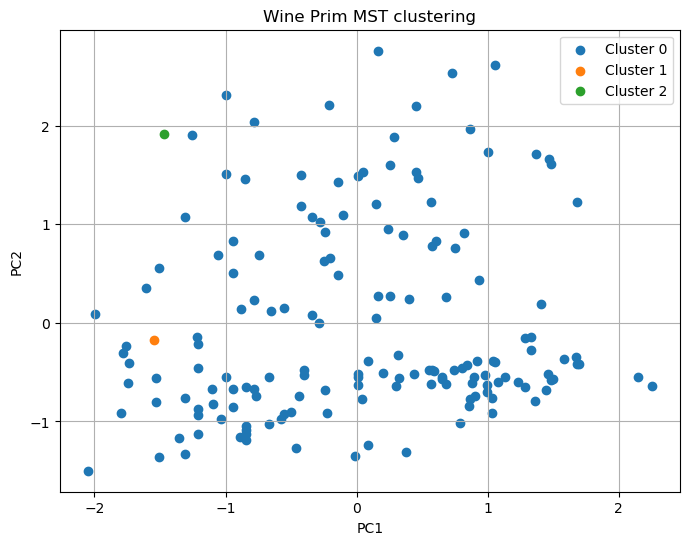
\includegraphics{/Users/danilakokin/Desktop/UPC/Semester3/OTDM/OTDM_Project_3/3/linprog/img/wine_prim_2d.png}
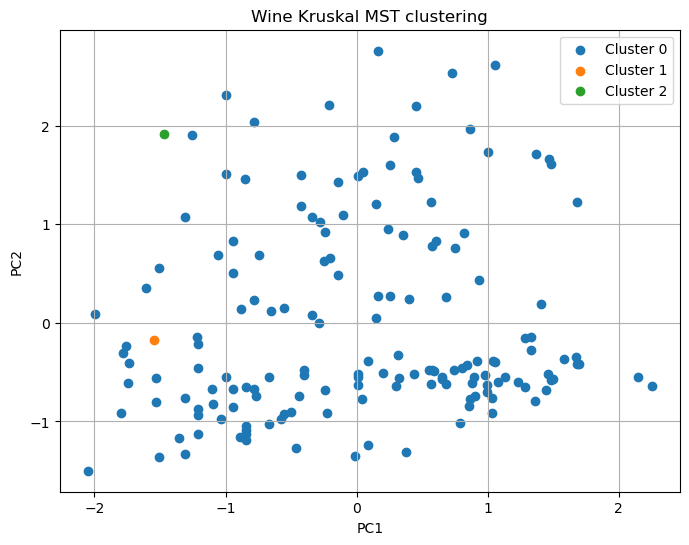
\includegraphics{/Users/danilakokin/Desktop/UPC/Semester3/OTDM/OTDM_Project_3/3/linprog/img/wine_kruskal_2d.png}
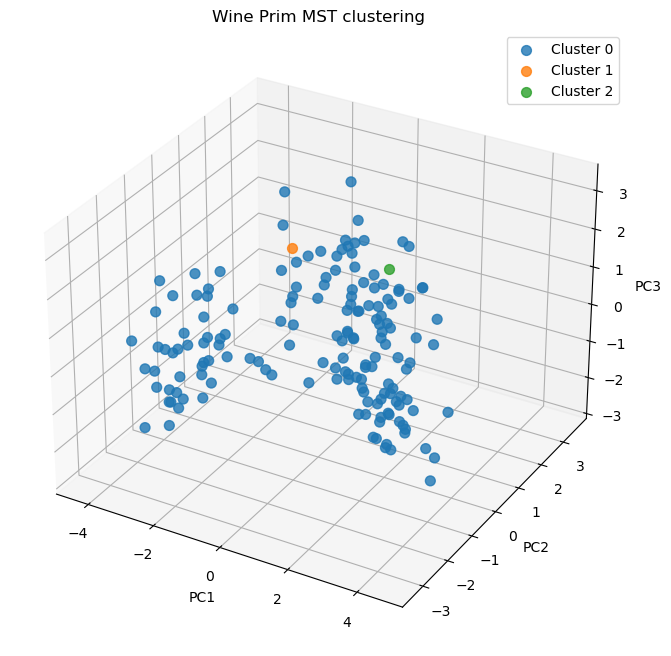
\includegraphics{/Users/danilakokin/Desktop/UPC/Semester3/OTDM/OTDM_Project_3/3/linprog/img/wine_prim_3d.png}
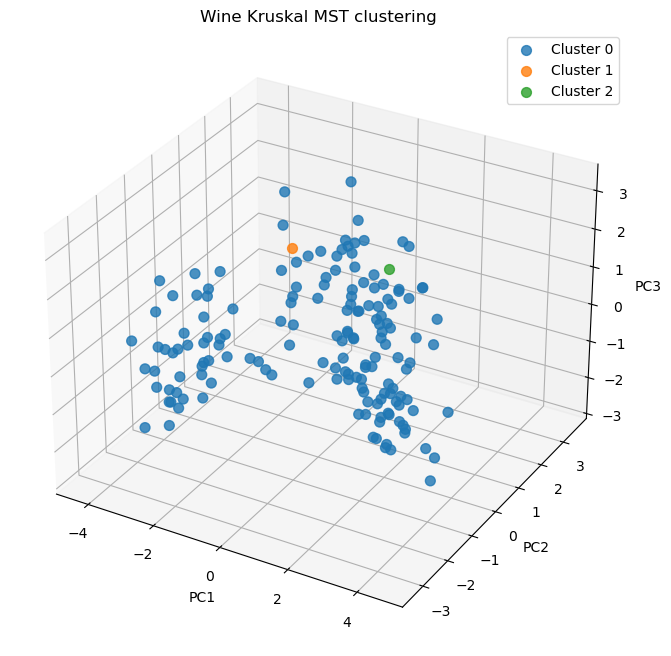
\includegraphics{/Users/danilakokin/Desktop/UPC/Semester3/OTDM/OTDM_Project_3/3/linprog/img/wine_kruskal_3d.png}

\subsection{7. A comparison of the two solutions obtained, in terms of
the objective function of the integer optimization problem. Optionally,
you may provide any other additional criteria for
comparison.}\label{a-comparison-of-the-two-solutions-obtained-in-terms-of-the-objective-function-of-the-integer-optimization-problem.-optionally-you-may-provide-any-other-additional-criteria-for-comparison.}

\subsection{8. Any other observation or comment you may want to add, or
any problem you had when performing the
assignment.}\label{any-other-observation-or-comment-you-may-want-to-add-or-any-problem-you-had-when-performing-the-assignment.}

Conclusion: \ldots{}

\section{Not to be included:}\label{not-to-be-included}

\begin{Shaded}
\begin{Highlighting}[]
\CommentTok{\#cd /home/julian/uni\_folder/OTDM/OTDM\_Project\_2/3/linprog/}
\end{Highlighting}
\end{Shaded}

(for generating script: cd
/home/julian/uni\_folder/OTDM/OTDM\_Project\_2/3/linprog/ python3
clean\_data\_linprog.py wine-clustering.csv 3 scaledWine.txt
matrixWine.txt ``,'')

\end{document}
